\section{UC20 - Impostazioni livelli per automatismo luminosità area}\label{uc:20}
\paragraph{Intenzione in contesto} L'attore primario desidera modificare uno dei due livelli che impostano l'automatismo dell'illuminazione in un'area. 

\paragraph{Attore primario} L'attore primario è l'utente gestore.
\paragraph{Precondizioni} L'attore primario è autenticato ed autorizzato dal sistema.
\paragraph{Post-condizioni} I livelli a cui l'area deve portare l'intensità luminosa sono stati impostati.
\paragraph{Scenario principale}
\begin{enumerate}
    \item L'attore primario sceglie a quale area apportare modifiche;
    \item l'attore imposta le modifiche relative ad \hyperref[uc:20.1]{UC20.1};
    \item l'attore imposta le modifiche relative ad \hyperref[uc:20.2]{UC20.2};
    \item le modifiche entrano in azione nel sistema. 
\end{enumerate}

\begin{figure}[H]
    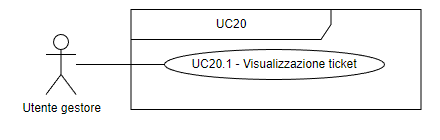
\includegraphics[width=\textwidth]{contenuti/img/casi_uso_grafici-uc20.png}
    \caption{UC20 in dettaglio}
    \label{fig:uc20}
\end{figure}

\subsection{UC20.1 - Impostazione livello superiore per automatismo luminosità area}\label{uc:20.1}
\paragraph{Intenzione in contesto} L'attore primario vuole impostare il livello a cui deve essere impostata l'illuminazione dell'area specifica in caso di movimento rilevato dai sensori del sistema.
\paragraph{Attore primario} L'attore primario è l'utente gestore.
\paragraph{Precondizioni} L'attore primario è autenticato ed autorizzato dal sistema.
\paragraph{Post-condizioni} Il livello superiore dell'illuminazione nell'area è impostato.
\paragraph{Scenario principale}
\begin{enumerate}
    \item L'attore primario dice al sistema a quale area desidera modificare il parametro;
    \item l'attore primario imposta il livello a cui dovrà trovarsi l'illuminazione in caso di rilevato movimento;
    \item il parametro viene impostato nel sistema.
\end{enumerate}

\subsection{UC20.2 - Impostazione livello inferiore per automatismo luminosità area}\label{uc:20.2}

\paragraph{Intenzione in contesto} L'attore primario vuole impostare il livello a cui deve essere impostata l'illuminazione dell'area specifica dopo che avviene un timeout dall'ultimo movimento rilevato dal sistema.
\paragraph{Attore primario} L'attore primario è l'utente gestore.
\paragraph{Precondizioni} L'attore primario è autenticato ed autorizzato dal sistema.
\paragraph{Post-condizioni} Il livello inferiore automatico dell'illuminazione nell'area è impostato.
\paragraph{Scenario principale}
\begin{enumerate}
    \item L'attore primario dice al sistema a quale area desidera modificare il parametro;
    \item l'attore primario imposta il livello a cui dovrà tornare l'area dopo che un determinato lasso di tempo è passato dall'ultimo movimento rilevato nell'area;
    \item il parametro viene impostato nel sistema.
\end{enumerate}